\documentclass{standalone}

\usepackage{fontspec}
\usepackage[mathrm=sym]{unicode-math}


\usepackage{tikz}
\usetikzlibrary{calc}
\usetikzlibrary{positioning}
\usetikzlibrary{arrows.meta}
\usetikzlibrary{shadings}
\usepackage[compat=1.1.0]{tikz-feynman}


\usepackage{xcolor}
\definecolor{cherenkov}{RGB}{87,202,255}
\colorlet{gamma}{red!80!black}
\colorlet{proton}{blue!80!black}

\usepackage{xparse}
\NewDocumentCommand{\pGamma}{}{\ensuremath{\symup{\gamma}}}
\NewDocumentCommand{\pP}{}{\ensuremath{\symup{e}^{+}}}
\NewDocumentCommand{\pE}{}{\ensuremath{\symup{e}^{-}}}

\usepackage{xstring}

\renewcommand\familydefault\sfdefault
\setsansfont{Fira Sans}
\setmathfont{Fira Math}




\IfEndWith*{\jobname}{_de}{
  \newcommand\primary{Primäres geladenes Teilchen}
  \newcommand\subshower{EM-Subschauer}
}{
  \newcommand\primary{Primary Cosmic Ray}
  \newcommand\subshower{EM-subshower}
}

\begin{document}

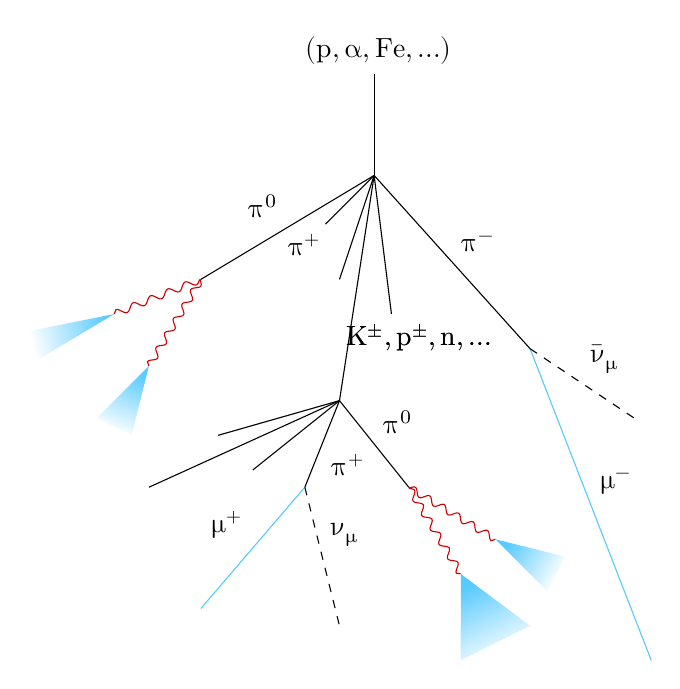
\begin{tikzpicture}[scale=2.2]
  \begin{feynman}
    \tikzfeynmanset{
      every photon={gamma, text=black},
      every scalar={draw=cherenkov}
      plain/.style={draw=darkgray},
      fermion/.style={draw=cherenkov},
      anti fermion/.style={draw=cherenkov},
    }

    \vertex (primary) at (0, 0.12) {\primary{} $(\symup{p}, \symup{α}, \mathup{Fe}, ...)$};
    \vertex (first) at (0, -0.6);

    \vertex (v_1_1) at (-1, -1.2);
    \vertex (v_1_2) at (-0.4, -1) {$\symup{\pi}^{+}$};
    \vertex (v_1_3) at (-0.2, -1.2);
    \vertex (v_1_4) at (-0.2, -1.9);
    \vertex (v_1_5) at (0.1, -1.4);
    \vertex (v_1_6) at (0.9, -1.6);

    \vertex (v_2_1) at (-1.5, -1.4);
    \vertex (v_2_2) at (-1.3, -1.7);

    \vertex (v_2_3) at (-0.9, -2.1);
    \vertex (v_2_4) at (-1.3, -2.4);
    \vertex (v_2_5) at (-0.7, -2.3);
    \vertex (v_2_6) at (-0.4, -2.4);
    \vertex (v_2_7) at (0.2, -2.4);

    \vertex (v_2_8) at (1.6, -3.4);
    \vertex (v_2_9) at (1.5, -2);

    \vertex (v_3_1) at (-1, -3.1);
    \vertex (v_3_2) at (-0.2, -3.2);
    \vertex (v_3_3) at (0.5, -2.9);
    \vertex (v_3_4) at (0.7, -2.7);

    \diagram* {
      (primary)  -- [plain] (first),

      (first)  -- [plain, edge label'=$\symup{\pi}^0$] (v_1_1),
      (first)  -- [plain] (v_1_2),
      (first)  -- [plain] (v_1_3),
      (first)  -- [plain] (v_1_4),
      (first)  -- [plain] (v_1_5),
      (first)  -- [plain, edge label=$\symup{\pi}^{-}$] (v_1_6),

      (v_1_1) -- [photon, edge label'=\pGamma] (v_2_1);
      (v_1_1) -- [photon, edge label=\pGamma] (v_2_2);

      (v_1_4) -- [plain] (v_2_3);
      (v_1_4) -- [plain] (v_2_4);
      (v_1_4) -- [plain] (v_2_5);
      (v_1_4) -- [plain, edge label=$\symup{\pi}^+$] (v_2_6);
      (v_1_4) -- [plain, edge label=$\symup{\pi}^0$] (v_2_7);

      (v_1_6) -- [fermion, edge label=$\symup{\mu}^{-}$] (v_2_8);
      (v_1_6) -- [scalar, edge label=$\bar{\symup{\nu}}_{\symup{\mu}}$] (v_2_9);

      (v_2_6) -- [anti fermion, edge label'=$\symup{\mu}^{+}$] (v_3_1);
      (v_2_6) -- [scalar, edge label=$\symup{\nu}_{\symup{\mu}}$] (v_3_2);

      (v_2_7) -- [photon, edge label'=\pGamma] (v_3_3);
      (v_2_7) -- [photon, edge label=\pGamma] (v_3_4);
    };
  \end{feynman}

  \shade[bottom color=white, top color=cherenkov, shading angle=-77] (v_2_1) -- (-2, -1.5) -- (-2, -1.7) -- cycle;
  \shade[bottom color=white, top color=cherenkov, shading angle=-22] (v_2_2) -- (-1.6, -2) -- (-1.4, -2.1) -- cycle;

  \shade[top color=cherenkov, shading angle=26] (v_3_3) -- (0.5, -3.4) -- (0.9, -3.2) -- cycle;
  \shade[top color=cherenkov, shading angle=60] (v_3_4) -- (1, -3) -- (1.1, -2.8) -- cycle;
  \node[rotate=35] at (-1.6, -1.65) {\subshower};
  \node[rotate=-40] at (0.87, -3.02) {\subshower};
  \node[anchor=140] at (v_1_5) {$\symup{K}^{\pm}, \symup{p}^{\pm}, \symup{n}, ...$};
  \node[anchor=140] at (v_1_5) {$\symup{K}^{\pm}, \symup{p}^{\pm}, \symup{n}, ...$};
\end{tikzpicture}
\end{document}
